\begin{center}
    \section*{\fontsize{20}{20}\selectfont Chapter 5}
\end{center}
\vspace{10mm}

\section{Standards, Constraints, and Milestones}

A good model is not enough for a farm tool. We also need to follow engineering standards, think about the environment and ethics, and be honest about the limits of the project. In this chapter we show how the project fits the United Nations Sustainable Development Goals (SDGs) and some software standards. We then look at the effect on society, ethics, the problems we faced and the 26-week timeline.

\subsection{Sustainability Standards}
The project supports five UN Sustainable Development Goals (SDGs). It also follows some basic software and testing standards.

\subsubsection*{Alignment with UN Sustainable Development Goals (SDGs)}
Table~\ref{tab:sdg_alignment} shows how our 8.64~MB model and the web application for farmers connect to five UN SDGs.

\begin{table}[htbp]
\caption{Alignment of the Proposed System with UN Sustainable Development Goals}
\label{tab:sdg_alignment}
\begin{center}
\begin{tabularx}{\textwidth}{| L{2.3cm} | L{3.6cm} | X |}
\hline
\textbf{UN SDG} & \textbf{Goal Title} & \textbf{How the Project Helps} \\
\hline
SDG 2 & Zero Hunger & The model finds late blight (\textit{Phytophthora}), fungal, bacterial and viral diseases early (93.51\% single-pass, 93.94\% with TTA). Farmers can act in time and save their harvest. \\
\hline
SDG 9 & Industry, Innovation, and Infrastructure & A small 8.64~MB model does better than a 118.55~MB ensemble. It runs on a light, open-source FastAPI/React web platform that anyone can reach. \\
\hline
SDG 12 & Responsible Consumption and Production & The app names the exact disease, and Gemini gives advice without doses. This helps farmers avoid spraying the whole field, so they waste less chemical and money. \\
\hline
SDG 13 & Climate Action & A small model uses less server energy than ensembles of more than 100~MB. It also helps farmers react quickly when the weather brings new disease outbreaks. \\
\hline
SDG 15 & Life on Land & Less fungicide and bactericide runoff is better for soil life, bees and the water near potato fields. \\
\hline
\end{tabularx}
\end{center}
\end{table}

\subsubsection*{Engineering and Software Standards}
\textit{Coding standard (PEP~8).} The training notebooks and the FastAPI backend follow PEP~8 style. The code is split into small functions, and settings are written in one clear place.

\textit{Reproducibility and export checks.} We fixed the random seed (\texttt{42}). The code checks that the hash-based split has no overlap. After training, automatic checks test the model, and the exported file is compared with the trained model ($\Delta_{\max} = 0.00 \times 10^{0}$). Because of this, anyone can repeat our runs and get the same numbers.

\textit{Data license and testing standard.} The field images are public, and we use them only for academic research, under their Kaggle license \cite{shabrina2024novel}. All four models are scored with the same standard multi-class metrics on the same held-out test set \cite{grandini2020metrics}.

\subsection{Impacts on Society}
The app can help farming communities in three ways.

\textit{Easy access to diagnosis.} Many small farmers cannot reach a plant doctor quickly. With our app, they can take a leaf photo in a phone browser and get a first diagnosis at once. They also see the Grad-CAM heatmap and get simple advice in Bengali or English.

\textit{Less money lost.} Serious diseases such as \textit{Phytophthora} late blight (0.94 recall) and \textit{Bacterial Disease} (1.00 recall) can be caught early. This stops bigger yield losses and saves money spent on the wrong treatment.

\textit{Less harm to the environment.} Fungicides do not work on viral diseases. If the app can tell a viral infection apart from a fungal or bacterial one, farmers spray less chemical for nothing, and less of it runs off into the land and water.

\subsection{Ethics}
We tried to reduce three risks: bias, wrong diagnosis and loss of privacy.

\textit{Bias from uneven classes.} There are $3.66$ times more \textit{Fungi} images than \textit{Healthy} images. Without care, the model could miss the small classes. We used capped class weights and picked checkpoints by macro-F1. As a result, recall is 100\% on \textit{Healthy} and 94\% on \textit{Phytophthora}. We also report the weak points openly, for example the 0.79 precision on \textit{Healthy}.

\textit{Risk of a wrong diagnosis.} Even at 93.51--93.94\% accuracy, the model will sometimes be wrong, and the farmer may then take the wrong action. So every screen of the web app shows a clear note (\textit{``AI-based preliminary classification---not a definitive diagnosis''}). The app shows the confidence score and the Grad-CAM overlay. When a case is uncertain, it asks the farmer to check with the local agricultural extension officer.

\textit{Privacy and safe use of the LLM.} We do not send any personal data or leaf photos to the outside LLM. Only the disease name and the confidence score go to Google Gemini. The API key is kept in an environment variable. The prompt has strict rules: Gemini must not make up chemical brand names or doses.

\subsection{Challenges}
We faced four main technical problems and solved them as follows.

\textit{Leakage between splits.} Burst photos of the same leaf could make the validation score look too good. We used 64-bit perceptual difference hashing ($\text{dHash} \le 10$), union-find grouping and \texttt{StratifiedGroupKFold}. After this, no photo group was shared between splits in any experiment.

\textit{Unstable fine-tuning.} In our first baseline, unfreezing the Batch Normalization layers of MobileNetV2 made the validation loss jump from $0.83$ to $2.63$. We fixed this by restoring the best Stage~1 head weights, keeping all BN layers frozen in the top 54 layers, and switching to AdamW with gradient clipping. The problem went away, and accuracy rose by 2.17 percentage points.

\textit{Saving and loading the models.} At first, custom Keras \texttt{Lambda} layers made the models hard to save, and evaluating inside the GPU strategy gave slightly different probabilities. We replaced the \texttt{Lambda} layers with built-in \texttt{Rescaling} and frozen $1 \times 1$ \texttt{Conv2D} layers, and we reloaded the checkpoints outside \texttt{MirroredStrategy}. After that, the exported files matched exactly ($0.00 \times 10^{0}$) for all four models.

\textit{Diseases that look alike.} \textit{Fungal Disease}, \textit{Phytophthora} and early lesions look very similar, especially on a busy soil background. This was still the main source of errors. It is the reason we added brightness augmentation and 4-view TTA.

\subsection{Timeline and Gantt Chart}
The project took 26 weeks. Phase~I (Weeks~1--13) covered planning, data work and model design. Phase~II (Weeks~14--26) covered training and comparing the models, tuning, web deployment and writing. Figures~\ref{fig:gantt1} and~\ref{fig:gantt2} show the Gantt charts.

\subsubsection{Phase I: Planning and System Design (Weeks 1--13)}
\begin{itemize}
    \item \textbf{Weeks 1--2:} We read papers on computer vision in farming, small CNNs, transfer learning, XAI and LLM advisors.
    \item \textbf{Weeks 3--5:} We prepared and checked the dataset, and wrote the leak-aware split (perceptual hash $\text{dHash} \le 10$ with \texttt{StratifiedGroupKFold}).
    \item \textbf{Weeks 6--10:} We designed the MobileNetV2 pipeline, the input format and the training augmentation.
    \item \textbf{Weeks 11--13:} We designed the three comparison pipelines (MultiNet-V3 Ensemble, InceptionV3 and NASNetMobile) and made them use the same setup.
\end{itemize}

\begin{figure}[!htbp]
\centering
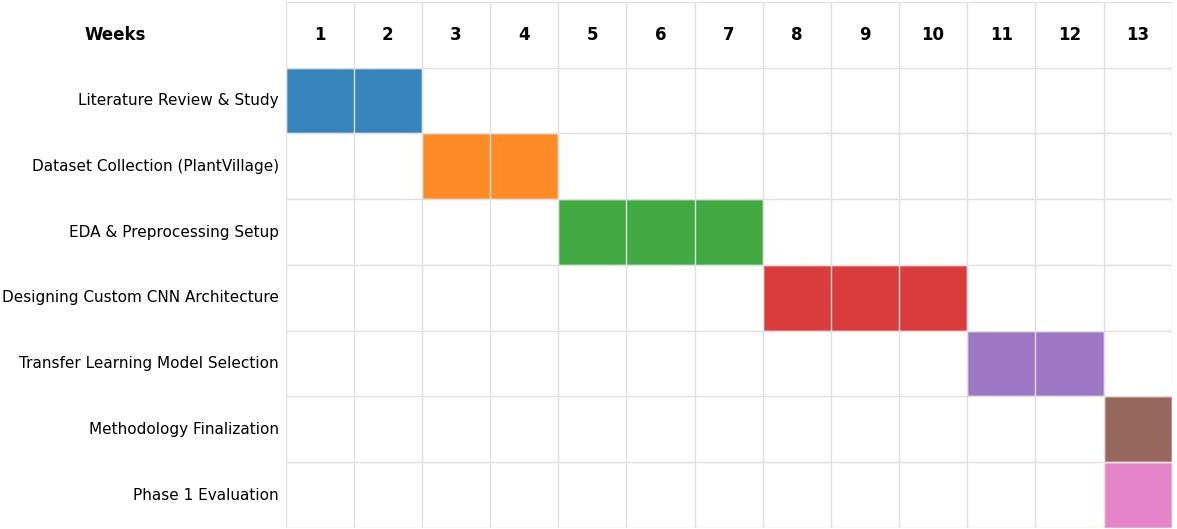
\includegraphics[width=0.95\textwidth]{image/docx_image26.jpeg}
\caption{Gantt Chart I -- Timeline for Planning, Data Preparation, and Model Design (Weeks 1--13).}
\label{fig:gantt1}
\end{figure}

\subsubsection{Phase II: Implementation, Benchmarking, Deployment, and Documentation (Weeks 14--26)}
\begin{itemize}
    \item \textbf{Weeks 14--17:} We trained all four models on two GPUs on Kaggle, checked the exported files and tuned the fine-tuning (frozen BN, AdamW, 4-view TTA).
    \item \textbf{Weeks 18--21:} We compared accuracy against size, checked Grad-CAM for each model, added the Gemini safety prompt and deployed the FastAPI/React web app.
    \item \textbf{Weeks 22--26:} We put together the tables, figures and chapters of the thesis, and prepared for the final defense.
\end{itemize}

\begin{figure}[!htbp]
\centering
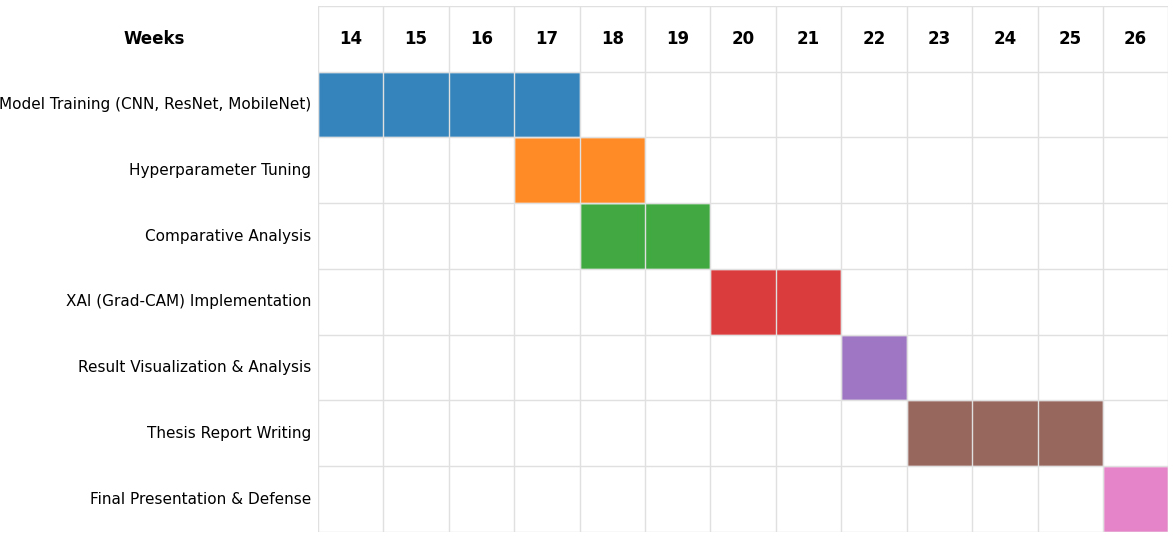
\includegraphics[width=0.95\textwidth]{image/docx_image27.png}
\caption{Gantt Chart II -- Timeline for Implementation, Benchmarking, Web Deployment, and Documentation (Weeks 14--26).}
\label{fig:gantt2}
\end{figure}
